\title{\textbf{Programming project :\\Secondary Structure Assignment}}
\author{
        H\'{e}l\`{e}ne Kabbech \\
        Bioinformatics master student, Paris Diderot University\\
}

\documentclass[12pt]{article}
\usepackage{geometry}
\usepackage{graphicx}
\usepackage{epstopdf} %%package to overcome problem with eps in pdf files

\geometry{
	a4paper,
	total={170mm,257mm},
	left=20mm,
	top=20mm,
}
\usepackage{listings}
\lstdefinestyle{myCustomMatlabStyle}{
	language=Matlab,
	numbers=left,
	stepnumber=1,
	numbersep=10pt,
	tabsize=4,
	showspaces=false,
	showstringspaces=false
}
\lstset{
	basicstyle=\scriptsize,
	style=myCustomMatlabStyle
}
\begin{document}
\maketitle

\section{Introduction}
As Kabsch and Sander did in the 80's, the aim of this project is to generate a pattern-recognition program which assign secondary structures to a protein by using the dictionary of protein secondary structures based on hydrogen-bonded and geometrical features extracted from atomic coordinates.

\section{Material \& Method}
\subsection{Programming}
The programming script is written in Python 3.6. The BioPython library (reference) is used to manage pdb files. The script is separated into three modules : classes (Residue and Nturn), Structure, Additional\_functions
GitHubMy project (documentation, script sources) is available online I used GitHub, a web-based hosting service for version control using Git
method dssp / reduce program / GitHub\\
In order to assign the secondary structure elements (SSE), we follow the strategy decribed in the article, which is priority \textbf{H} ($\alpha$-helix), \textbf{B} (isolated $\beta$-bridge), \textbf{E} (extended strand), \textbf{G} ($\textrm{3}_\textrm{10}$-helix), \textbf{I} ($\pi$-helix), \textbf{T} (H-bonded turn) and \textbf{S} (bend).  

\subsection{Input files}
Protein Data Bank files
Reduce program (add reference) is used to add hydrogen coordinates into a pdb file.
\subsection{Output parameters}
The program different parameters describe a residue (see \textbf{Annexe})\\
\begin{itemize}
	\item\textbf{RESIDUE :} Residue sequence number and chain identifier
	\item\textbf{AA :} One letter amino acid code.
	\item\textbf{STRUCTURE} (first column in STRUCTURE block) : Compromise summary of secondary structure, intended to approximate crystallographers' intuition, based on columns 19-38, which are the principal result of DSSP analysis of the atomic coordinates.
	\item\textbf{BP1 BP2 :} Residue number of first and second bridge partner
	\item\textbf{TCO :} Cosine of angle between C=O of residue i and C=O of residue i-1. For alpha-helices, TCO is near +1, for beta-sheets TCO is near -1. Not used for structure definition.
	\item\textbf{KAPPA :} Virtual bond angle (bend angle) defined by the three C-alpha atoms of residues i-2, i, i+2. Used to define bend (structure code 'S').
	\item\textbf{ALPHA :} Virtual torsion angle (dihedral angle) defined by the four C-alpha atoms of residues i-1, i, i+1, i+2. Used to define chirality (structure code '+' or '-').
	\item\textbf{PHI PSI :} IUPAC peptide backbone torsion angles
	\item\textbf{X-CA Y-CA Z-CA :} C-alpha atom coordinates
\end{itemize}

\subsection{Example}
1bta, 1itv

\section{Results}
The dssp program is run with two example.
First the 1BTA pdb file, then a more complex pdb 1ITV 

\subsection{A simple example}
1BTA is Its structure consist of a sheet (3 beta-strands parallels) and 4 alpha-helices.
By comparing our result with the mkdssp program, we obtain the good result with a isolated beta-bridge
\section{Conclusion}
We worked hard, and achieved very little.
\clearpage
\bibliographystyle{abbrv}
\bibliography{main}
W. Kabsch and C.Sander, Biopolymers 22 (1983) 2577-2637
\\
\begin{figure}[h!]
	\centering
	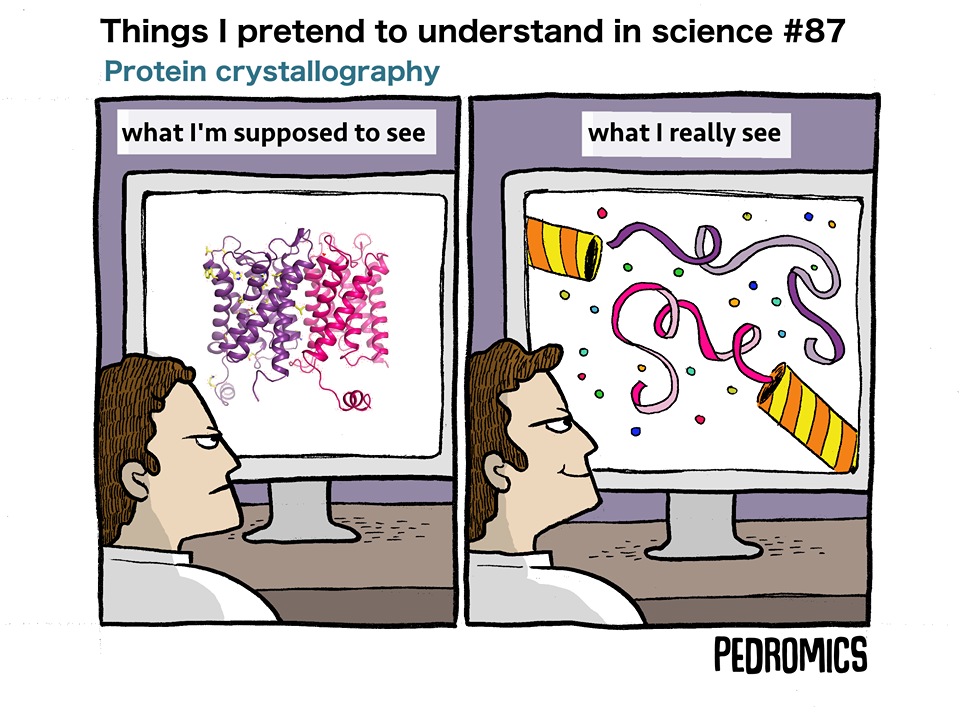
\includegraphics[totalheight=8cm]{img/pedromics.png}
	\label{fig:verticalcell}
\end{figure}
\clearpage
\section{Annexe}

\begin{lstlisting}
./dssp.py -h
Usage: dssp.py [options]

Options:
--version             show program's version number and exit
-h, --help            show this help message and exit
-i FILE, --input=FILE
                      the file name of a PDB formatted file containing the
                      protein structure data
-o FILE, --output=FILE
                      the  file  name  of  a  DSSP  file to create

./dssp.py -i data/1bta.pdb
==== Secondary Structure Assignment using DSSP method ====
DATE		2018-09-17
REFERENCE	W. KABSCH AND C.SANDER, BIOPOLYMERS 22 (1983) 2577-2637
HEADER		RIBONUCLEASE INHIBITOR                  1994-05-09
COMPND		MOL_ID: 1; MOLECULE: BARSTAR; CHAIN: A; ENGINEERED: YES; 
SOURCE		MOL_ID: 1; ORGANISM_SCIENTIFIC: BACILLUS AMYLOLIQUEFACIENS; ORGANISM_TAXID: 1390; 
AUTHOR		M.J.LUBIENSKI,M.BYCROFT,S.M.V.FREUND,A.R.FERSHT
  #  RESIDUE AA STRUCTURE BP1 BP2    TCO  KAPPA ALPHA  PHI   PSI    X-CA   Y-CA   Z-CA
    1    1 A K              0   0   0.000 360.0 360.0 360.0-171.7   -7.5    5.2    9.2
    2    2 A K  E     -a   50   0  -0.957 360.0-169.5-133.8 153.7   -3.8    5.5    8.5
    3    3 A A  E     -a   51   0  -0.933   5.4-159.9-134.7 157.3   -1.1    3.4    6.8
    4    4 A V  E     -a   52   0  -0.926   5.9-160.1-144.5 118.6    2.7    3.8    6.8
    5    5 A I  E     -a   53   0  -0.740  11.7-170.1-100.1  93.0    5.1    2.2    4.2
    6    6 A N  E >>  -a   54   0  -0.684   4.7-172.9 -83.5 104.2    8.5    2.2    5.9
    7    7 A G  B 34 S+B    9   0   0.931  79.7  70.5 -64.8 -43.3   11.0    1.3    3.1
    8    8 A E  T 34 S+     0   0   0.812 111.2  36.3 -44.5 -25.9   13.9    1.0    5.5
    9    9 A Q  B <4 S+B    7   0   0.868  92.5  99.6 -94.9 -47.2   12.1   -2.1    6.7
   10   10 A I     <  +     0   0  -0.075  41.7 176.6 -41.3 133.7   10.6   -3.4    3.4
   11   11 A R        -     0   0   0.480  64.2 -14.5-119.2 -11.8   12.8   -6.3    2.2
   12   12 A S  S  > S-     0   0  -0.982  82.9 -77.3-174.2 175.9   10.7   -7.3   -0.9
   13   13 A I  H  > S+     0   0   0.951 127.9  57.2 -56.6 -45.7    7.3   -6.8   -2.5
   14   14 A S  H  > S+     0   0   0.940 105.2  51.7 -50.8 -45.4    5.9   -9.3   -0.0
   15   15 A D  H  > S+     0   0   0.933 106.8  54.1 -57.9 -43.3    7.1   -7.0    2.7
   16   16 A L  H  X S+     0   0   0.978 112.3  41.4 -55.2 -56.5    5.3   -4.1    1.0
   17   17 A H  H  X S+     0   0   0.740 110.3  64.2 -64.5 -18.6    2.0   -5.9    0.9
   18   18 A Q  H  X S+     0   0   0.979 107.7  36.0 -70.2 -55.2    2.9   -7.0    4.5
   19   19 A T  H  X S+     0   0   0.935 117.5  53.5 -65.2 -41.3    2.9   -3.6    6.0
   20   20 A L  H  X S+     0   0   0.903 108.1  52.9 -59.0 -35.8   -0.0   -2.6    3.8
   21   21 A K  H  X>S+     0   0   0.915 111.4  44.2 -66.9 -42.1   -1.8   -5.7    5.1
   22   22 A K  H  <5S+     0   0   0.993 120.2  39.8 -67.3 -57.4   -1.2   -4.6    8.7
   23   23 A E  H  <5S+     0   0   0.986 124.9  37.7 -52.3 -66.1   -2.2   -1.0    8.2
   24   24 A L  H  <5S-     0   0   0.680 104.4-138.4 -61.2 -14.8   -5.1   -1.9    5.9
   25   25 A A  T  <5 -     0   0   0.947  32.7-172.8  55.0  47.6   -5.7   -4.9    8.2
   26   26 A L      < -     0   0  -0.276  28.8 -88.3 -69.5 161.1   -6.3   -7.1    5.1
   27   27 A P    >   -     0   0   0.135  42.3 -99.3 -57.4-179.7   -7.5  -10.6    5.5
   28   28 A E  T 3  S+     0   0   0.714 123.6  58.2 -79.9 -18.5   -5.1  -13.5    6.0
   29   29 A Y  T 3  S+     0   0   0.276  71.5 159.2 -93.5  13.8   -5.4  -14.4    2.3
   30   30 A Y    <   -     0   0  -0.088  34.8-151.8 -38.4 105.9   -4.3  -10.9    1.2
   31   31 A G        -     0   0   0.584  14.6-148.0 -64.0  -5.5   -3.2  -11.8   -2.4
   32   32 A E        +     0   0   0.533  59.2 118.6  50.1   3.6   -0.7   -8.9   -2.0
   33   33 A N  S  > S-     0   0  -0.245  83.5-105.6 -84.8-176.0   -1.2   -8.3   -5.8
   34   34 A L  H  > S+     0   0   0.879 122.2  52.6 -76.7 -36.9   -2.6   -5.1   -7.3
   35   35 A D  H  > S+     0   0   0.864 117.0  38.0 -66.2 -36.2   -5.9   -6.9   -8.0
   36   36 A A  H  > S+     0   0   0.958 115.3  50.2 -80.8 -55.9   -6.2   -8.1   -4.4
   37   37 A L  H >X S+     0   0   0.945 117.0  44.5 -45.1 -50.8   -4.8   -5.0   -2.7
   38   38 A W  H 3X S+     0   0   0.981 104.5  59.7 -58.5 -56.4   -7.3   -3.0   -4.8
   39   39 A D  H 3< S+     0   0   0.812 108.4  50.8 -44.0 -26.1  -10.1   -5.5   -4.1
   40   40 A C  H X<>S+     0   0   0.948 110.2  44.4 -79.7 -51.4   -9.4   -4.4   -0.6
   41   41 A L  H 3<5S+     0   0   0.950 117.0  45.6 -58.8 -49.5   -9.5   -0.6   -1.1
   42   42 A T  T 3<5S+     0   0   0.445 137.1  10.0 -75.7   3.9  -12.6   -0.8   -3.2
   43   43 A G  T < 5S+     0   0  -0.002 130.8  26.0-177.1  60.5  -14.3   -3.2   -0.7
   44   44 A W  T   5S+     0   0  -0.122  87.7  83.5 177.1 -66.6  -12.5   -3.8    2.6
   45   45 A V  S   <S-     0   0  -0.236  74.1-125.7 -58.4 149.6  -10.3   -0.9    3.9
   46   46 A E        -     0   0  -0.847  39.5-110.6-102.7 132.4  -12.2    1.8    5.8
   47   47 A Y  S    S+     0   0  -0.696  90.6  61.5-114.5 169.3  -11.7    5.4    4.6
   48   48 A P  S    S+     0   0   0.380  81.4 177.7 -61.4 136.7  -10.9    8.1    4.7
   49   49 A L  E     - c   0  84  -0.825  22.4-142.4-113.2 156.5   -7.5    6.3    4.8
   50   50 A V  E     -ac   2  85  -0.941   5.5-163.5-117.3 138.5   -4.0    7.8    4.9
   51   51 A L  E     -ac   3  86  -0.706   6.7-175.6-120.0  81.8   -1.1    6.2    3.0
   52   52 A E  E     -ac   4  87  -0.526  12.7-169.6 -77.6  83.2    2.0    7.7    4.5
   53   53 A W  E     -ac   5  88  -0.650   2.5-170.5 -79.7 111.4    4.4    6.1    2.1
   54   54 A R  E     +a    6   0  -0.740  66.4  12.3-100.4 150.0    8.0    6.6    3.4
   55   55 A Q  S  > S+     0   0   0.977  75.3 172.3  49.9  68.7   11.1    5.7    1.3
   56   56 A F  T >4 S+     0   0   0.990  74.6  35.2 -73.9 -66.7    9.0    5.2   -1.9
   57   57 A E  T >> S+     0   0   0.885 118.0  56.0 -56.2 -35.2   11.8    4.8   -4.6
   58   58 A Q  H 3> S+     0   0   0.870 110.1  44.4 -66.4 -32.2   13.8    2.9   -1.9
   59   59 A S  H << S+     0   0   0.203 110.8  59.4 -94.7  17.7   10.8    0.6   -1.5
   60   60 A K  H <4>S+     0   0   0.721 102.9  45.3-111.5 -38.1   10.5    0.3   -5.3
   61   61 A Q  H ><5S+     0   0   0.992 101.0  62.9 -70.6 -62.9   14.0   -1.0   -6.3
   62   62 A L  T 3<5S+     0   0   0.779 118.8  32.6 -33.5 -32.0   14.4   -3.8   -3.7
   63   63 A T  T 3 5S-     0   0  -0.471 103.0-130.4-128.6  62.6   11.3   -5.3   -5.4
   64   64 A E  T < 5S+     0   0   0.326  96.9   3.8 -12.4 107.0   11.7   -4.2   -9.0
   65   65 A N  T   <S+     0   0   0.874 104.4 124.7  73.7  32.1    8.3   -2.8   -9.8
   66   66 A G  T  > S+     0   0   0.939  72.3  21.6 -89.1 -69.2    7.2   -3.3   -6.2
   67   67 A A  H  > S+     0   0   0.716 111.9  68.3 -77.8 -21.6    6.0   -0.1   -4.6
   68   68 A E  H  > S+     0   0   0.795 103.2  48.0 -71.3 -21.9    5.1    1.9   -7.8
   69   69 A S  H  > S+     0   0   0.956 108.6  48.6 -81.4 -55.3    2.2   -0.6   -8.4
   70   70 A V  H  X S+     0   0   0.931 112.0  52.4 -52.0 -43.2    0.5   -0.7   -5.0
   71   71 A L  H  X S+     0   0   0.949 103.5  56.7 -59.2 -45.3    0.7    3.1   -5.0
   72   72 A Q  H  X S+     0   0   0.891 109.3  47.4 -52.7 -38.1   -1.0    3.1   -8.4
   73   73 A V  H  X S+     0   0   0.830 110.4  51.0 -75.0 -30.8   -3.8    1.2   -6.8
   74   74 A F  H  X S+     0   0   0.881 116.9  39.6 -74.7 -35.0   -4.0    3.5   -3.8
   75   75 A R  H  X S+     0   0   0.874 115.3  52.1 -80.2 -37.3   -4.3    6.6   -6.0
   76   76 A E  H  X S+     0   0   0.958 112.5  45.1 -63.3 -46.7   -6.5    4.8   -8.5
   77   77 A A  H  <>S+     0   0   0.931 109.5  55.9 -62.6 -38.8   -8.8    3.9   -5.6
   78   78 A K  H ><5S+     0   0   0.859 107.6  50.2 -58.4 -30.9   -8.4    7.5   -4.5
   79   79 A A  H 3<5S+     0   0   0.788  94.7  70.7 -77.3 -28.8   -9.7    8.2   -7.9
   80   80 A E  T 3<5S-     0   0   0.585 129.3 -91.6 -65.8  -6.6  -12.6    5.8   -7.4
   81   81 A G  T < 5S+     0   0   0.209  87.8 133.5 113.3 -14.1  -14.0    8.4   -5.0
   82   82 A C      < -     0   0  -0.209  60.3-126.0 -63.9 160.5  -12.3    6.9   -1.9
   83   83 A D        +     0   0  -0.492  47.3 152.7-109.3  65.3  -10.5    9.3    0.4
   84   84 A I  E     -c   49   0  -0.688  39.5-144.7 -94.3  87.9   -7.0    7.7    0.7
   85   85 A T  E     -c   50   0  -0.284  15.8-146.8 -52.9  98.9   -4.8   10.7    1.4
   86   86 A I  E     -c   51   0  -0.577  18.1-174.3 -73.4 114.6   -1.7    9.7   -0.6
   87   87 A I  E     -c   52   0  -0.865   2.5-173.3-114.2 101.2    1.3   11.0    1.3
   88   88 A L  E      c   53   0  -0.800 360.0 360.0 -96.8 106.7    4.6   10.3   -0.7
   89   89 A S              0   0  -0.879 360.0 360.0-109.0 360.0    7.6   11.3    1.4

\end{lstlisting}
	
\end{document}